\documentclass[12pt,a4paper]{article}
\usepackage[utf8x]{inputenc}
\usepackage[english,hebrew]{babel}
\usepackage{graphicx}
\usepackage{verbatim}
\usepackage{url}
\usepackage{float}

\usepackage{tikz}
\usetikzlibrary{external,positioning,through,calc,intersections}
\tikzexternalize[prefix=tikz/]

\textwidth=15.5cm
\textheight=23cm
\topmargin=0pt
\headheight=0pt
\oddsidemargin=2em
\headsep=0pt
\renewcommand{\baselinestretch}{1.1}
\setlength{\parskip}{0.3\baselineskip plus 1pt minus 1pt}
\parindent=0pt

\addtolength{\jot}{3pt}

\begin{document}
\thispagestyle{empty}

\selectlanguage{hebrew}

\begin{center}
\textbf{\Huge%
האם משולשים עם אותו שטח\\
\bigskip
ואותו היקף חופפים?%
}

\bigskip

\bigskip

\textbf{\Large מוטי בן-ארי}

\bigskip

\textbf{\Large המחלקה להוראת המדעים}

\bigskip

\textbf{\Large מכון ויצמן למדע}

\bigskip

\selectlanguage{english}
\url{http://www.weizmann.ac.il/sci-tea/benari/}
\end{center}

\bigskip
\bigskip

\begin{center}
\selectlanguage{english}
\copyright{}\  2018 by Moti Ben-Ari.

\end{center}

\selectlanguage{english}

{\small This work is licensed under the Creative Commons Attribution-ShareAlike 3.0 Unported License. To view a copy of this license, visit \url{http://creativecommons.org/licenses/by-sa/3.0/} or send a letter to Creative Commons, 444 Castro Street, Suite 900, Mountain View, California, 94041, USA.}

\bigskip

\begin{center}

\includegraphics[width=.2\textwidth]{../by-sa.png}
\end{center}

\selectlanguage{hebrew}

\newpage

%%%%%%%%%%%%%%%%%%%%%%%%%%%%%%%%%%%%%%%%%%%%%%%%%%%%%%%%%%%%%%%

האם משולשים עם אותו שטח ואותו היקף חופפים? לא בהכרח: למשולשים עם הצלעות
$(17,25,28)$
ו-%
$(20,21,27)$
היקף
$70$
ושטח 
$210$.
\L{Barabash [1]}
מראה שנתון משולש שווה-צלעות, קיימים משולשים לא חופפים עם אותו היקף ואותו שטח. אולם, ההוכחה שלה לא כוללת בנייה. מסמך זה )המבוסס על 
\L{[2]}(
מראה שנתון משולש עם אורכי צלעות רציונליים, ניתן לבנות משולש לא-חופף עם אורכי צלעות רציונליים, ועם אותו היקף ושטח.

הבנייה גם מספקת הוכחה אלגנטית לנוסחה של הרון לשטח של משולש.


\selectlanguage{english}

[1] Barabash, Marita. A Non-Visual Counterexample in Elementary Geometry. \textit{The College Mathematics Journal} 36(5), 2005.

[2] McCallum, William. \textit{A tale of two triangles: Heron triangles and elliptic curves}, 2012, \url{http://blog.kleinproject.org/?p=4}.


\selectlanguage{hebrew}

\section{%
ממשולשים לעקומות אליפטיות%
}

איור%
~\ref{fig.incenter}
מציג את 
$O$, 
מרכז המעגל החסום על ידי המשולש
$\triangle ABC$, 
שהוא החיתוך של חוצי הזווית של שלושת הזוויות. כדי להוכיח שחוצי הזוויות נחתכים בנקודה אחת, שימו לב שחוצה זווית הוא אוסף הנקודות במרחק שווה מהצלעות, ולהפך, אוסף הנקודות במרחק שווה מהצלעות מגדיר חוצה זווית. הנקודה
$O$
נמצאת במרחק שווה מ-%
$AB$,
ו-% 
$AC$,
וגם במרחק שווה מ-%
$AB$
ו-%
$BC$.
מכאן ש-%
$O$
נמצאת במרחק שווה מ-%
$AC$
ו-%
$BC$,
ולכן היא נמצאת על חוצה הזווית של 
$\angle C$.

\vspace*{-6ex}

\begin{figure}[H]
\begin{center}
\selectlanguage{english}
\begin{tikzpicture}[baseline=-6mm,scale=2.2]
% Draw base and path two lines at known angles
\draw (0,0) coordinate (a) node[xshift=-6pt] {$A$} -- (0:6) coordinate (b) node[xshift=6pt] {$B$};
\path[name path=ac] (a) -- +(50:4);
\path[name path=bc] (b) -- +(150:5);
% Get their intersection and draw lines between vertices
\path[name intersections={of=ac and bc,by=c}];
\node[above] at (c) {$C$};
\draw (a) -- (c) -- (b) -- (a);
% Label angles with tick marks
\draw (a) ++(0:5mm) arc (0:50:5mm);
\draw (a) ++(10:4.5mm) -- +(10:1mm);
\draw (a) ++(15:4.5mm) -- +(15:1mm);
\draw (a) ++(35:4.5mm) -- +(35:1mm);
\draw (a) ++(40:4.5mm) -- +(45:1mm);
\draw (b) ++(150:7mm) arc (150:180:7mm);
\draw (b) ++(157.5:6.5mm) -- +(157.5:1mm);
\draw (b) ++(172.5:6.5mm) -- +(172.5:1mm);
\draw (c) ++(230:5mm) arc (230:330:5mm);
\draw (c) ++(250:4.5mm) -- +(250:1mm);
\draw (c) ++(255:4.5mm) -- +(255:1mm);
\draw (c) ++(260:4.5mm) -- +(260:1mm);
\draw (c) ++(300:4.5mm) -- +(300:1mm);
\draw (c) ++(305:4.5mm) -- +(305:1mm);
\draw (c) ++(310:4.5mm) -- +(310:1mm);
% Path bisectors of two lines
\path[name path=bia] (a) -- +(25:3.5);
\path[name path=bib] (b) -- +(165:5);
% Intersection of angle bisectors
\path [name intersections={of=bia and bib,by=center}];
% Draw angle bisectors to center
\draw (a) -- (center);
\draw (c) -- (center);
\draw (b) -- (center);
% Draw radii
\draw (center) -- node[left] {$r$} ($(a)!(center)!(b)$) node[below,yshift=-2pt] {$C'$} coordinate (ap);
\draw (center) -- node[left,yshift=-4pt] {$r$} ($(a)!(center)!(c)$) node[above left] {$B'$} coordinate (bp);
\draw (center) -- node[right] {$r$} ($(b)!(center)!(c)$) node[above right] {$A'$} coordinate (cp);
% Draw dots
\fill (center) circle (1pt) node[right,xshift=4pt,yshift=4pt] {$O$};
\fill (a) circle (1pt);
\fill (b) circle (1pt);
\fill (c) circle (1pt);
\fill (ap) circle (1pt);
\fill (bp) circle (1pt);
\fill (cp) circle (1pt);
% Draw right angle squares
\draw (ap) -- ++(90:4pt) -- ++(0:4pt) -- ++(-90:4pt);
\draw (bp) -- ++(-40:4pt) -- ++(-130:4pt) -- ++(-220:4pt);
\draw (cp) -- ++(-30:4pt) -- ++(-120:4pt) -- ++(-210:4pt);
\end{tikzpicture}
\selectlanguage{hebrew}
\caption{%
מרכז המעגל החסום על ידי משולש}%
\label{fig.incenter}
\end{center}
\end{figure}

\vspace*{-6ex}

הורידו גבהים מ-%
$O$
לצלעות. נוצרים זוגות של משולשים 
\textbf{ישר זווית}
\[\{\triangle AOB', \triangle AOC'\}, \{\triangle BOA', \triangle BOC'\}, \{\triangle COA', \triangle COB'\}\,,
\]
כי לכל זוג יתר משותף והזוויות שנוצרו על ידי חוצי הזוויות שוות. מכאן שאורכי הגבהים שווים, ונסמן אותם ב-%
$r$.

איור%
~\ref{fig.altitudes}
מציג את הצלעות
$a,b,c$
המחולקות לקטעי קו
$u,v,w$,
והזוויות
$\alpha/2,\beta/2,\gamma/2$
של שלושת הזוגות של משולשים מסביב למרכז המעגל החסום
$O$.
השטח של 
$\triangle ABC$
הוא סכום השטחים של 
$\triangle AOC, \triangle BOC, \triangle AOB$. $r$
הוא הגובה של כל המשלושים ולכן השטח הוא:
\begin{equation}
A = \frac{1}{2}(w+v)r + \frac{1}{2}(v+u)r + \frac{1}{2}(u+w)r = \frac{1}{2}\cdot 2(u+v+w)r = rs\,, \label{eq.area1}
\end{equation}
כי מחצית ההיקף הוא:
\begin{equation}
s=\frac{1}{2}\cdot 2 (u+v+w)=u+v+w\,.\label{eq.semi}
\end{equation}

\vspace*{-8ex}

\begin{figure}[H]
\begin{center}
\selectlanguage{english}
\begin{tikzpicture}[baseline=-6mm,scale=2.2]
% Draw base and path two lines at known angles
\draw (0,0) coordinate (a) node[xshift=-8pt] {$A$} -- (0:6) coordinate (b) node[xshift=6pt] {$B$};
\path[name path=ac] (a) -- +(50:4);
\path[name path=bc] (b) -- +(150:5);
% Get their intersection and draw lines between vertices
\path[name intersections={of=ac and bc,by=c}];
\node[above] at (c) {$C$};
\draw (a) -- node[right] {$b$} (c) -- node[below] {$a$} (b) -- node[above] {$c$} (a);
% Path bisectors of two lines
\path[name path=bia] (a) -- +(25:3.5);
\path[name path=bib] (b) -- +(165:5);
% Intersection of angle bisectors
\path [name intersections={of=bia and bib,by=center}];
% Draw angle bisectors to center
\draw (a) -- (center);
\draw (c) -- (center);
\draw (b) -- (center);
% Labels of angles
\node[above,xshift=3pt,yshift=14pt] at (center) {$\displaystyle\frac{\gamma}{2}$};
\node[above left,xshift=-4pt,yshift=14pt] at (center) {$\displaystyle\frac{\gamma}{2}$};
\node[above right,xshift=8pt,yshift=-5pt] at (center) {$\displaystyle\frac{\beta}{2}$};
\node[below right,yshift=-6pt] at (center) {$\displaystyle\frac{\beta}{2}$};
\node[left,xshift=-12pt,yshift=3pt] at (center) {$\displaystyle\frac{\alpha}{2}$};
\node[below left,xshift=2pt,yshift=-6pt] at (center) {$\displaystyle\frac{\alpha}{2}$};
% Draw radii
\draw (center) -- node[near end,left] {$r$} ($(a)!(center)!(b)$) coordinate (cp) node[below,yshift=-2pt] {$C'$};
\draw (center) -- node[left,near end,yshift=-4pt] {$r$} ($(a)!(center)!(c)$) coordinate (bp) node[above left] {$B'$};
\draw (center) -- node[right,near end] {$r$} ($(b)!(center)!(c)$) coordinate (ap) node[above right] {$A'$};
\fill (ap) circle (1pt);
\fill (bp) circle (1pt);
\fill (cp) circle (1pt);
\fill (a) circle (1pt);
\fill (b) circle (1pt);
\fill (c) circle (1pt);
% Draw dot at center
\fill (center) circle (1pt);
% Labels of line segments
\path (a) -- node[below,yshift=-2pt] {$u$} (cp);
\path (a) -- node[left,xshift=-2pt]  {$u$} (bp);
\path (b) -- node[below,yshift=-2pt] {$v$} (cp);
\path (b) -- node[above,xshift=2pt] {$v$} (ap);
\path (c) -- node[above,xshift=-2pt] {$w$} (bp);
\path (c) -- node[above,xshift=2pt] {$w$} (ap);
\end{tikzpicture}
\selectlanguage{hebrew}
\caption{%
הזוויות וקטעי הקו הנוצרים על ידי הגבהים}%
\label{fig.altitudes}
\end{center}
\end{figure}

\vspace*{-6ex}

ניתן לחשב את האורכים של 
$u,v,w$
מהזוויות ו-%
$r$:
\begin{eqnarray}
\tan \frac{\alpha}{2} &=& \frac{u}{r}\label{eq.alpha}\\
\tan \frac{\beta}{2} &=& \frac{v}{r}\label{eq.beta}\\
\tan \frac{\gamma}{2} &=& \frac{w}{r}\label{eq.gamma}\,.
\end{eqnarray}
כעת ניתן לבטא את
$s$
במונחים של טנגוסים:
\[
s = u+v+w = r\tan \frac{\alpha}{2}+r\tan \frac{\beta}{2}+r\tan \frac{\gamma}{2} = r\left(\tan \frac{\alpha}{2}+\tan \frac{\beta}{2}+\tan \frac{\gamma}{2}\right)\,,
\]
ולפי משוואה%
~\L{\ref{eq.area1}}
השטח הוא:
\begin{equation}
A = rs = r^2\left(\tan \frac{\alpha}{2}+\tan \frac{\beta}{2}+\tan \frac{\gamma}{2}\right)\,.\label{eq.area2}
\end{equation}
מ-%
$A=rs$
אנו יודעים ש-%
$r=A/s$,
ולכן ניתן לבטא את משוואה%
~\L{\ref{eq.area2}}
כ-:
\begin{equation}
\tan \frac{\alpha}{2}+\tan \frac{\beta}{2}+\tan \frac{\gamma}{2} = \frac{A}{r^2} = \frac{A}{(A/s)^2} = \frac{s^2}{A}\,.\label{eq.area3}
\end{equation}
סכום הזוויות
$\alpha,\beta,\gamma$
הוא
$2\pi$,
ולכן:
\begin{eqnarray}
\gamma &=& 2\pi - (\alpha + \beta)\\
\gamma/2 &=& \pi - (\alpha/2 + \beta/2)\\
\tan\gamma/2 &=& \tan(\pi - (\alpha/2 + \beta/2))\\
&=& -\tan (\alpha/2 + \beta/2)\\
\tan\gamma/2 &=& \frac{\tan\alpha/2 + \tan\beta/2}{\tan\alpha/2 \, \tan\beta/2-1}\,.\label{eq.tangent1}
\end{eqnarray}
הנה הוכחה של הנוסחה לטנגוס של סכום של שתי זוויות:
\begin{eqnarray}
\tan (\theta+\phi) &=& \frac{\sin(\theta+\phi)}{\cos(\theta+\phi)}\\
&=&\frac{\sin\theta\cos\phi+\cos\theta\sin\phi}{\cos\theta\cos\phi-\sin\theta\sin\phi}\\
&=&\frac{\displaystyle\frac{\sin\theta}{\cos\theta}+\frac{\sin\phi}{\cos\phi}}{\displaystyle 1-\frac{\sin\theta\sin\phi}{\cos\theta\cos\phi}}\label{eq.tangent2}\\
\tan (\theta+\phi) &=&\frac{\tan\theta + \tan \phi}{1-\tan\theta\tan\phi}\,,\label{eq.tangent3}
\end{eqnarray}
כאשר משוואה%
~\L{\ref{eq.tangent2}}
מתקבלת על ידי חילוק ב-%
$\cos\theta\cos\phi$.

נפשט את הסימון על ידי הגדרת נעלמים עבור הטנגוסים:
\begin{eqnarray*}
x&=&\tan \frac{\alpha}{2}\\
y&=&\tan \frac{\beta}{2}\\
z&=&\tan \frac{\gamma}{2}\,.
\end{eqnarray*}
לפי משוואה%
~\L{\ref{eq.tangent1}}
ניתן להחליף את
$z=\tan\gamma/2$
בביטוי עם 
$x,y$:
\begin{equation}
z = \frac{x+y}{xy-1}\,.\label{eq.xy1}
\end{equation}
עם סימון זה, משוואה
~\L{\ref{eq.area3}}
היא:
\begin{equation}
x+y+\frac{x+y}{xy-1}=\frac{s^2}{A}\,.\label{eq.xy2}
\end{equation}
אם נתונים ערכים קבועים של 
$A$
ו-%
$s$,
האם קיים מספר פתרונות  למשוואה%
~\L{\ref{eq.xy2}}?

עבור משולש ישר-הזווית
$(3,4,5)$:
\begin{equation}
\frac{s^2}{A} = \frac{\left(\frac{1}{2}(3+4+5)\right)^2}{\frac{1}{2}\cdot 3\cdot 4} = \frac{6^2}{6}=6\,.
\end{equation}
אם קיים פתרון נוסף למשוואה:
\begin{equation}
x+y+\frac{x+y}{xy-1}=6\,,\label{eq.elliptic0}
\end{equation}
אז קיים משולש נוסף עם שטח
$6$
ומחצית ההיקף
$6$.
ניתן לבטא את משוואה%
~\L{\ref{eq.elliptic0}}
כ-:
\begin{equation}
x^2y + xy^2 -6xy + 6 = 0\,.\label{eq.elliptic}
\end{equation}
זו משוואה עבור
\textbf{עקומה אליפטית}.
\L{Andrew Wiles}
השתמש בעקומות אליפטיות בהוכחה של המשפט האחרון של
\L{Fermat}.
משתמשים בעקומות גם בהצפנה עם מפתח ציבורי.

\section{פתרון המשוואה לעקומה האליפטית}

איור%
~\L{\ref{fig.elliptic}}
מראה חלק מהגרף של משוואה%
~\L{\ref{eq.elliptic}}.
כל נקודה בעקומה הסגורה ברביע הראשון היא פתרון. אנו מעוניינים רק בנקודות ברביע הראשון כי אורכי הצלעות חייבים להיות חיוביים. הנקודות 
$A,B,D$
מתאימות למשולש
$(3,4,5)$
כפי שנראה בהמשך. כדי למצוא פתרונות 
\textbf{רציונליים}
נוספים, נשתמש ב-%
\textbf{שיטת שני סקנטים}
\L{(\textit{method of two secants})}.%
\footnote{\L{McCallum [2]}
כותב שיש מספר אינסופי של פתרונות רציונליים.}
\begin{figure}[H]
\selectlanguage{english}
\begin{center}
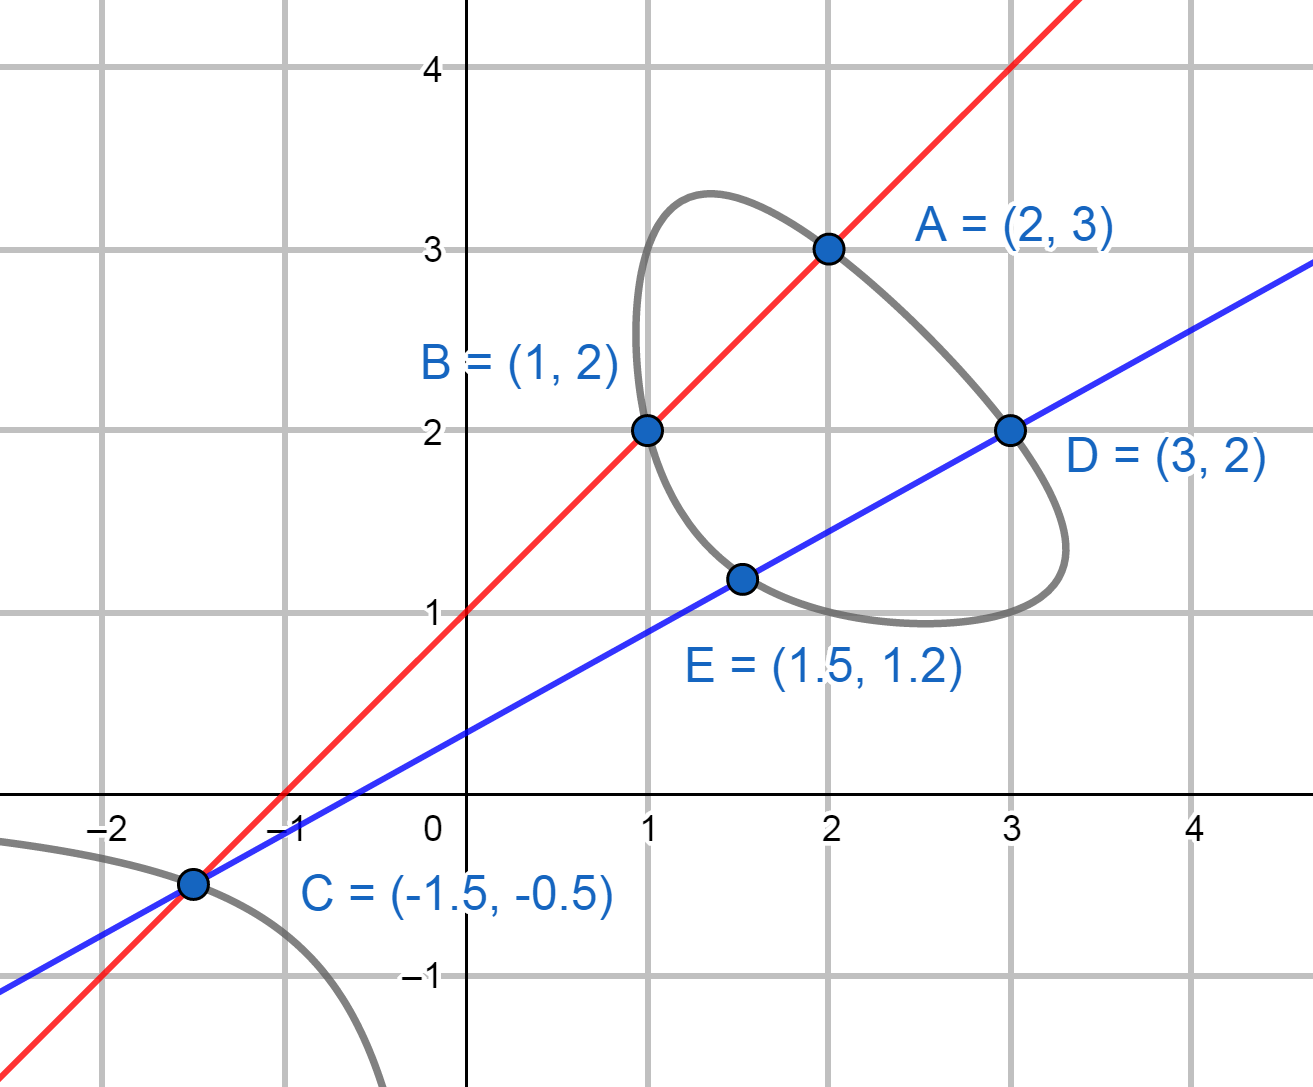
\includegraphics[width=.7\textwidth]{elliptic1}
\end{center}
\selectlanguage{hebrew}
\caption{%
הגרף של
$x^2y + xy^2 -6xy + 6 = 0$
עם שני סקנטים}%
\label{fig.elliptic}
\end{figure}

\vspace*{-4ex}
צייר סקנט דרך הנקודות
$A=(2,3)$
ו-%
$B=(1,2)$.
נראה שהוא חותך את העקומה ב-%
$C=(-1.5,-0.5)$,
אבל הנקודה איננה פתרון כי ערכי הקואורדינטות שליליים. אם נצייר סקנט שני מ-%
$C$
ל-%
$D=(3,2)$,
החיתוך שלו עם העקומה ב-%
$E$
כן מהווה פתרון נוסף.%
\footnote{$(1.5,1.2)$
הוא קירוב המוצג על ידי גיאוגברה. בהמשך נחשב את הקואורדינטות המדוייקות של
$E$.}

המשוואה של הקו )האדום( דרך 
$A,B$
היא
$y=x+1$. 
נציב עבור 
$y$
במשוואה%
~\L{\ref{eq.elliptic}}:
\[
x^2(x+1) + x(x+1)^2 -6x(x+1) +6 =0\,
\]
ונפשט:
\[
2x^3 -3x^2 -5x +6 =0\,.
\]
מהנקודות
$A,B$,
אנו יודעים שני שורשים
$x=2,x=1$,
כך שאפשר לפרק את הפולינום מדרגה שלוש כך:
\[
(x-2)(x-1)(ax+b)=0\,,
\]
כאשר רק השורש השלישי לא ידוע. נכפיל את הגורמים ונראה מיד ש-%
$a$,
המקדם של הגורם מדרגה שלוש
$x^3$,
חייב להיות
$2$,
ו-%
$2b$,
הקבוע, חייב להיות
$6$.
לכן, הגורם השלישי הוא
$2x+3$
ומכאן שהשורש השלישי הוא
$x=-\frac{3}{2}$.
נחשב
$y=x+1=-\frac{1}{2}$.
הקואורדינטות של הנקודה
$C$
הן
$(-\frac{3}{2},-\frac{1}{2})$.

כעת נצייר  סקנט שני )בכחול( דרך 
$C$
ו-%
$D=(3,2)$.
המשוואה של הקו היא:
\begin{equation}
y = \frac{5}{9}x + \frac{1}{3}\,.\label{eq.second-secant}
\end{equation}
נציב עבור 
$y$
במשוואה 
~\L{\ref{eq.elliptic}}:
\[
x^2\left(\frac{5}{9}x + \frac{1}{3}\right) + x\left(\frac{5}{9}x + \frac{1}{3}\right)^2 -6x\left(\frac{5}{9}x + \frac{1}{3}\right) +6 =0\,,
\]
ונפשט:
\[
\frac{70}{81}x^3 - \frac{71}{27}x^2 - \frac{17}{9}x +6 =0\,.
\]
שוב יש לנו שני שורשים
$x=3,x=-\frac{3}{2}$,
וניתן לפרק את הפולינום מדרגה שלוש כ:
\[
(x-3)(x+\frac{3}{2})(ax+b)=0\,.
\]
נשווה את המקדם של 
$x^3$
ונשווה את הקובע ונקבל:
\[
\frac{70}{81}x - \frac{4}{3}=0\,,
\]
ולכן:
\[
x=\frac{81}{70}\cdot \frac{4}{3}= \frac{27\cdot 4}{70} = \frac{54}{35}\,.
\]
נחשב את
$y$
ממשוואה
~\L{\ref{eq.second-secant}}
והקואורדינטות של
$E$
הן:
\[
\left(\frac{54}{35}, \frac{25}{21}\right)\,.
\]
לבסוף, נחשב את
$z$
ממשוואה
~\L{\ref{eq.xy1}}:
\[
z=\frac{x+y}{xy-1}=%
\displaystyle\left(\frac{54}{35} + \frac{25}{21}\right)%
 \, / \,%
\displaystyle\left(\frac{54}{35}\frac{25}{21}-1\right)=%
\frac{2009}{615} = \frac{49}{15}\,.
\]

\section{מפתורונות לעקומה האליפטית למשולשים}

מ-%
$x,y,z$, $a,b,c$, 
ניתן לחשב את אורכי הצלעות של המשולש
$\triangle ABC$:
\begin{eqnarray*}
a&=&w+v = r(z+y)=(z+y)\\
b&=&u+w= r(x+z)=(x+z)\\
c&=&u+v=r(x+y)=(x+y)\,,
\end{eqnarray*}
כי
$\displaystyle r=\frac{A}{s}=\frac{6}{6}=1$.

עבור הפתרון 
$A=(2,3)$
של העקומה האליפטית, ערכו של
$z$
הוא:
\[
z=\frac{x+y}{xy-1}=\frac{2+3}{2\cdot 3-1}=1\,,
\]
והצלעות של המשולש הם:
\begin{eqnarray*}
a &=& z+y = 1+3 = 4\\
b &=& x+z = 2+1=3\\
c &=& x+y = 2+3=5\,,
\end{eqnarray*}
המשולש ישר-זווית עם
$s=A=6$.
חישוב הצלעות המתאימים ל-%
$B$
ן-%
$D$
נותן את אותו משולש.

עבור
$E$:
\begin{eqnarray*}
a &=& z+y = \frac{49}{15} + \frac{25}{21} = \frac{156}{35}\\
b &=& x+z = \frac{54}{35} + \frac{49}{15} = \frac{101}{21}\\
c &=& x+y = \frac{54}{35} + \frac{25}{21}  = \frac{41}{15}\,,
\end{eqnarray*}
ואני בטוח שמצאת ערכים אלה בניסוי וטעייה!

נבדוק את התוצאה. מחצית ההיקף היא:
\[
s=\frac{1}{2}\left(\frac{156}{35} + \frac{101}{21}+\frac{41}{15}\right) = \frac{1}{2}\left(\frac{468+505+287}{105}\right) = \frac{1}{2}\left(\frac{1260}{105}\right)= 6\,,
\]
וניתן לחשב את השטח באמצעות הנוסחה של הרון:
\begin{eqnarray*}
A &=& \sqrt{s(s-a)(s-b)(s-c)}\\
&=& \sqrt{6 \left(6-\frac{156}{35}\right) \left(6-\frac{101}{21}\right) \left(6-\frac{41}{15}\right)}\\
&=& \sqrt{6 \cdot \frac{54}{35}\cdot \frac{25}{21} \cdot \frac{49}{15}}\\
&=& \sqrt{\frac{396900}{11025}}\\
&=& \sqrt{36} = 6\,.
\end{eqnarray*}

\section{הוכחה של הנוסחה של הרון}

אם
$\phi+\theta+\psi=\pi$,
הנוסחה של סכום שלושת הזוויות היא:
\begin{equation}
\tan\phi+\tan\theta+\tan\psi = \tan\phi\tan\theta\tan\psi\,. \label{eq.triple}
\end{equation}
ההוכחה היא מיידית ממשוואה
~\L{\ref{eq.tangent3}}:
\begin{eqnarray*}
\tan\psi &=& \tan (\pi-(\phi+\theta))\\
&=& -\tan (\phi+\theta)\\
&=& \frac{\tan\phi+\tan\theta}{\tan\phi\tan\theta-1}\\
\tan\phi\tan\theta\tan\psi-\tan\psi&=& \tan\phi+\tan\theta\\
\tan\phi\tan\theta\tan\psi &=&\tan\phi+\tan\theta+\tan\psi\,.
\end{eqnarray*}
ממשוואות 
~\L{\ref{eq.alpha}--\ref{eq.area2}}
ו-%
$r=A/s$:
\begin{eqnarray*}
A &=& r^2\left(\tan \frac{\alpha}{2}+\tan \frac{\beta}{2}+\tan \frac{\gamma}{2}\right)\\
&=&r^2\left(\tan \frac{\alpha}{2}\tan \frac{\beta}{2}\tan \frac{\gamma}{2}\right)\\
&=&r^2\left(\frac{u}{r}\frac{v}{r}\frac{w}{r}\right)\\
&=&\frac{u\,v\,w}{r}\\
&=&\frac{s}{A}\,u\,v\,w\\
A^2&=&s\,u\,v\,w\,.
\end{eqnarray*}
ממשוואה
~\L{\ref{eq.semi}}
והגדרת
$a,b,c,u,v,w$
באיור%
~\L{\ref{fig.altitudes}}:
\begin{eqnarray*}
s - a &=& (u+v+w) - (w+v) = u\\
s - b &=& (u+v+w) - (u+w) = v\\
s - c &=& (u+v+w) - (u+v) = w\,,
\end{eqnarray*}
אנו מקבלים את הנוסחה של הרון:
\begin{eqnarray*}
A^2 &=& s\,u\,v\,w\\
&=& s(s-a)(s-b)(s-c)\\
A &=& \sqrt{s(s-a)(s-b)(s-c)}\,.
\end{eqnarray*}


\end{document}

